%!TEX encoding = UTF-8 Unicode
%!TEX root = ../compendium.tex

\chapter{Integrerad utvecklingsmiljö}\label{appendix:ide}

\section{Vad är en IDE?}

\section{Kojo}\label{appendix:kojo}

\subsection{Installera Kojo}

\href{http://www.kogics.net/kojo-download}{www.kogics.net/kojo-download}

\subsection{Använda Kojo}

\begin{table}[h]
\caption{Några av sköldpaddans funktioner. Se även \href{http://lth.se/programmera}{lth.se/programmera}}
\vspace{1em}\small
\begin{tabular}{lll}
\emph{Svenska} & \emph{Engelska} & \emph{Vad händer?}\\ \hline
\tt fram     & \tt forward     & Paddan går 25 steg frammåt.           \\
\tt fram(50) & \tt forward(50) & Paddan går 50 steg frammåt.           \\
\tt höger    & \tt right       & Paddan vrider sig 90 grader åt höger. \\
\code+upprepa(10){???}+ & \code+repeat(10){???}+  & Repetition av ??? 10 gånger. \\
\end{tabular}
\end{table}

\noindent Koden för den svenska paddans api finns här:
\href{https://bitbucket.org/lalit\_pant/kojo/src/tip/src/main/scala/net/kogics/kojo/lite/i18n/svInit.scala?at=default\&fileviewer=file-view-default\#svInit.scala-26}{bitbucket.org/lalit\_pant/kojo/}

\section{Eclipse och ScalaIDE}\label{appendix:ide:eclipse}

\subsection{Installera Eclipse och ScalaIDE}\label{appendix:ide:eclipse:install}

\subsection{Använda Eclipse och ScalaIDE}\label{appendix:ide:eclipse:use}

\subsubsection{Ladda ner och importera projekt från kursens workspace}

TODO: skriv mer här

\begin{itemize}
\item Ladda ner kursens workspace här: \url{http://cs.lth.se/pgk/workspace}
\item Packa upp filen på lämpligt ställe.
\item Starta Eclipse med ScalaIDE-plugin (för installation se \ref{appendix:ide:eclipse:install}).
\item Bläddra till biblioteket du nyss packade upp, ungefär som i \ref{fig:eclipse:ide:open}
\item Högerklicka i package explorer och välj import
\item blablablabla
\end{itemize}

TODO: skriv mer här
  
\begin{figure}[H]
\centering
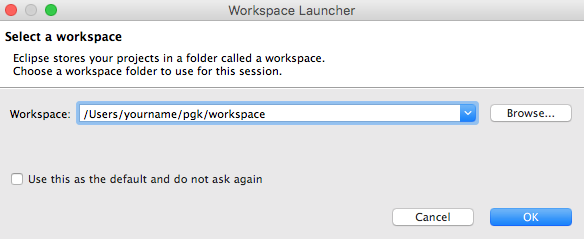
\includegraphics[width=0.7\textwidth]{../img/pirates/selectws.png}
\caption { \emph{Öppna workspace.} Bläddra fram till kursens workspace och klicka OK. }
\label{fig:eclipse:ide:open}
\end{figure}
